%Dies ist ein Test- testen testen
%!TeX spellcheck = de_DE

%  ******************************************************************************
%  * @file      tex/Anhang                                                      *
%  * @author    Mario Hesse                                                     *
%  * @version   v0.1.0                                                          *
%  * @date      31.01.2019                                                      *
%  ******************************************************************************



% ------
\appendix % Ändert die Nummerierung

% Schaltpläne
% -----------

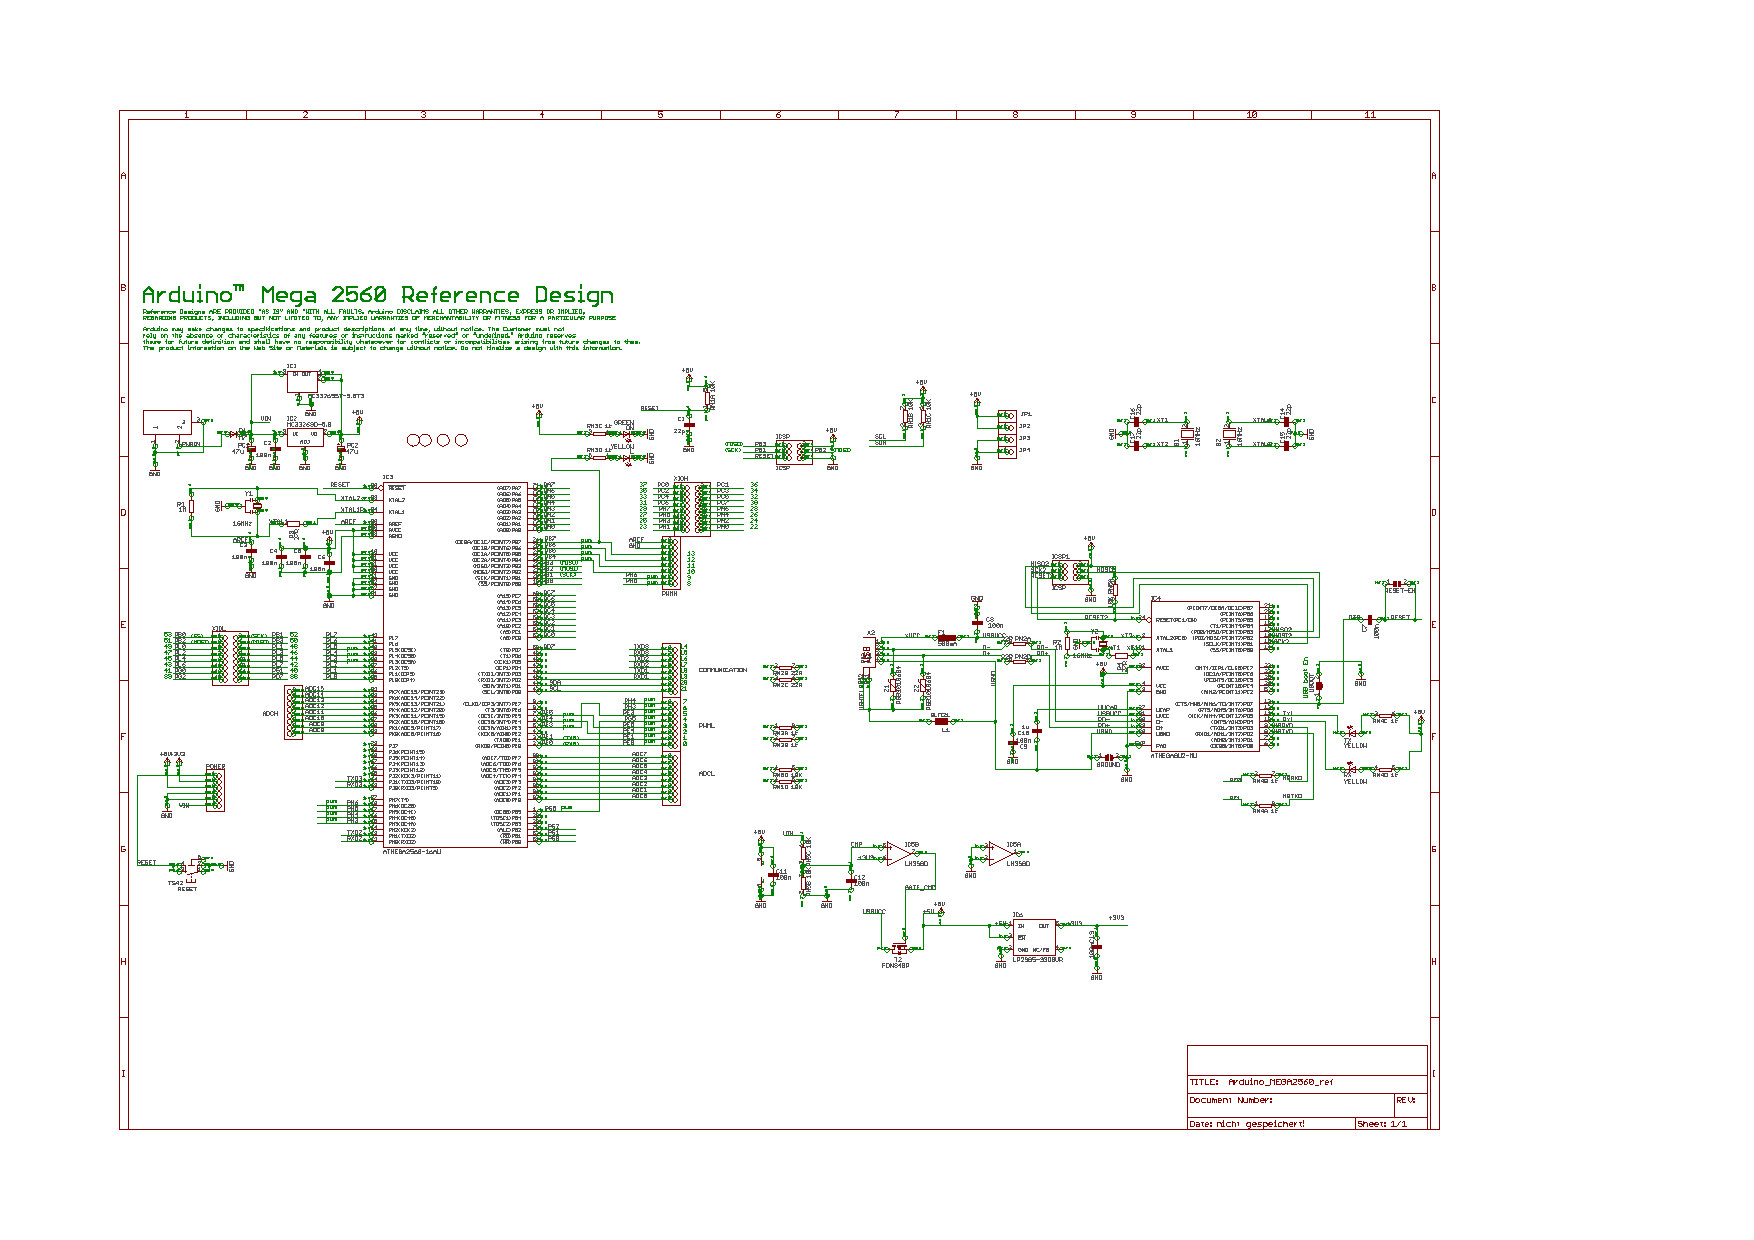
\includepdf[pagecommand={\section{Schaltpläne} \label{sec:Schaltplaene} \subsection{Arduino} \label{sec:sch-Arduino}}, angle=90, scale=0.9]{app/Arduino-sch.pdf}




% Platinenlayout
% --------------

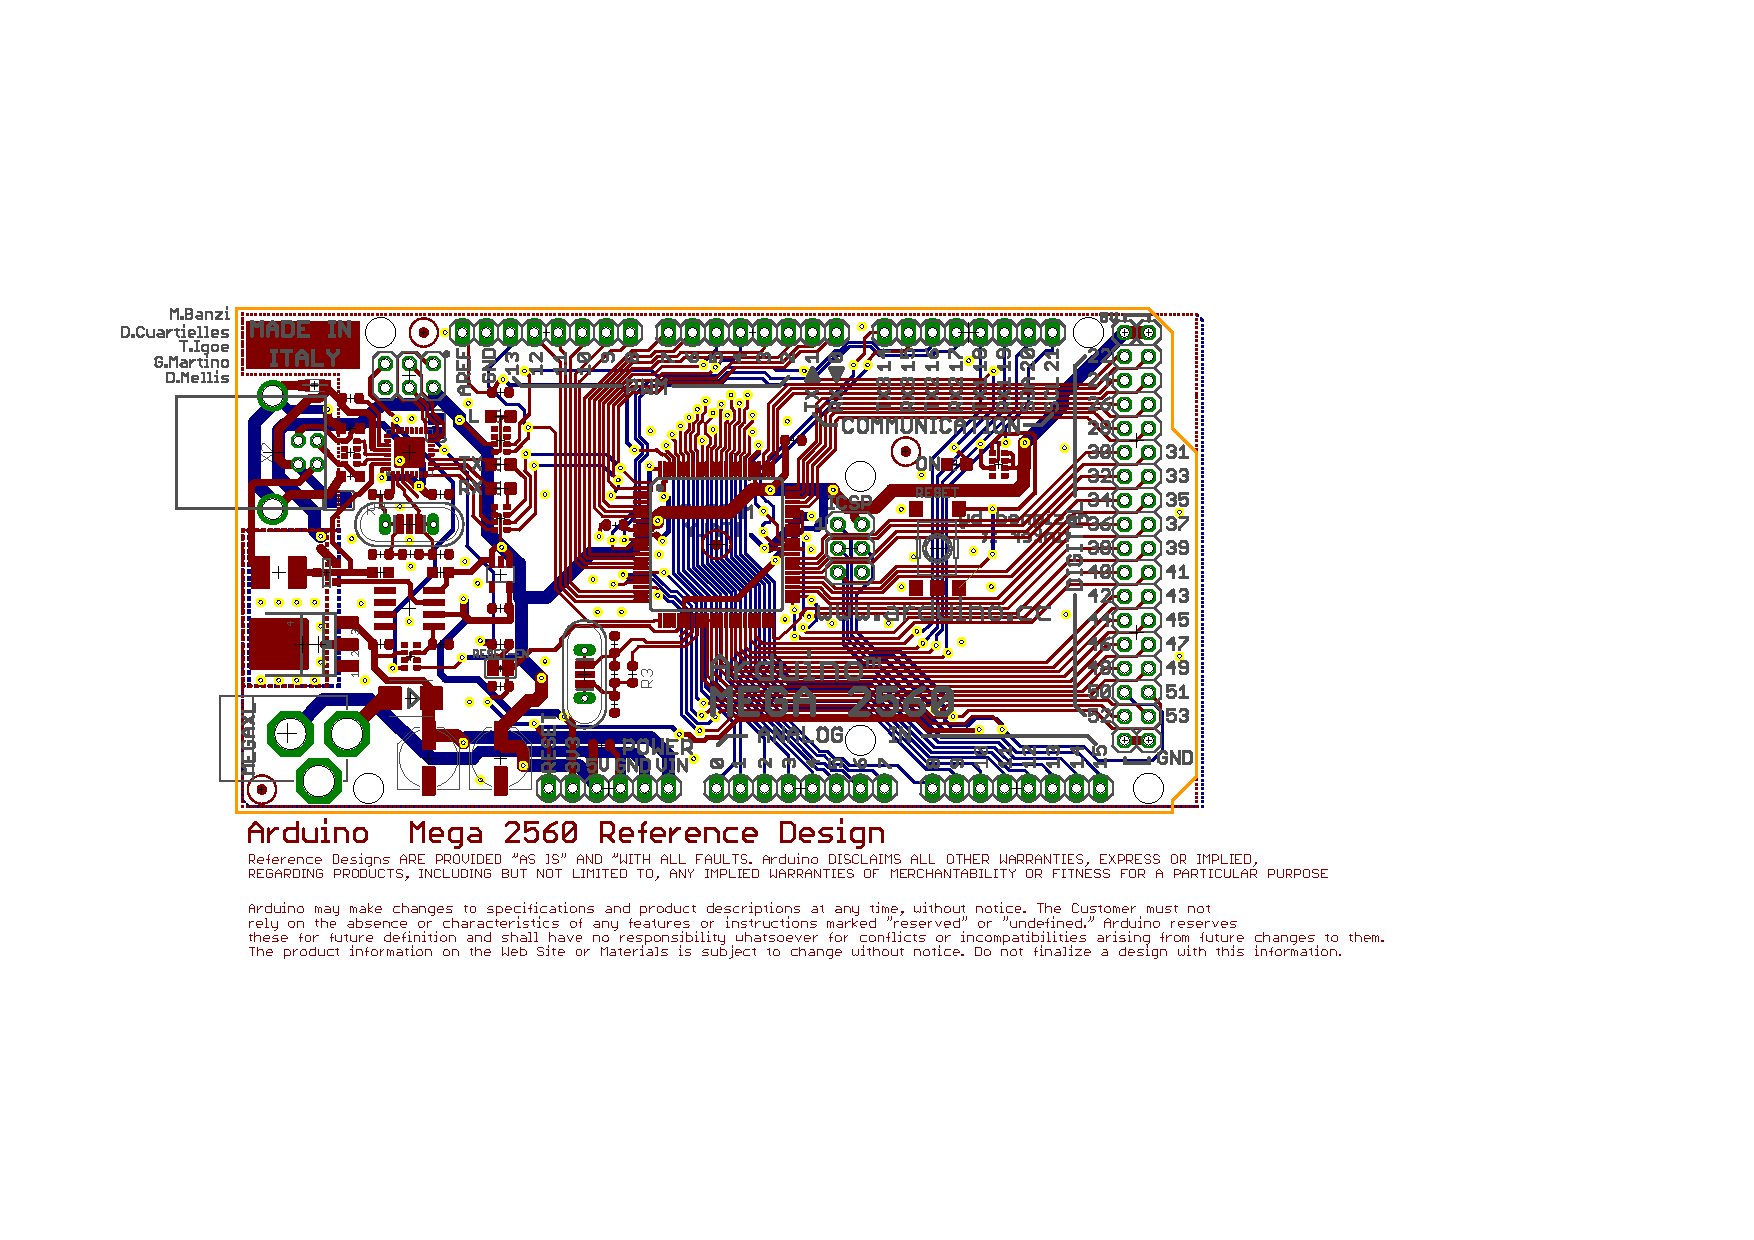
\includepdf[pagecommand={\section{Boardlayouts} \label{sec:Platinenlayout} \subsection{Arduino} \label{sec:brd-Arduino}}, angle=90, scale=0.8]{app/Arduino-brd.pdf}



% Verbindung der Platinen
% -----------------------
%\section{Verbindung der Platinen}



% Messdaten
% ---------
%\section{Messdaten}



% Datenblätter
% ------------
%\section{Datenblätter}



% Inhaltsverzeichnis der beiliegenden CD
% --------------------------------------
\clearpage 
%\includepdf[pagecommand={\section{Inhaltsverzeichnis der beiliegenden CD} \mario{Inhaltsverzeichnis CD fertig machen !}}, scale=0.7]{chapter/InhaltsverzeichnisCd.pdf}

\section{Inhaltsverzeichnis der beiliegenden CD}

\begin{forest}
	for tree={
		font=\ttfamily,
		grow'=0,
		child anchor=west,
		parent anchor=south,
		anchor=west,
		calign=first,
		edge path={
			\noexpand\path [draw, \forestoption{edge}]
			(!u.south west) +(7.5pt,0) |- node[fill,inner sep=1.25pt] {} (.child anchor)\forestoption{edge label};
		},
		before typesetting nodes={
			if n=1
			{insert before={[,phantom]}}
			{}
		},
		fit=band,
		before computing xy={l=15pt},
	}
	[	
		[1-Masterarbeit
			[Abbildungen]
			[Masterarbeit.pdf]
		]
		[2-Hardware
			[Datenblätter]
			[Eagle
				[Schaltung 1]
				[Schaltung 2]
				[\dots]
			]
		]
		[3-Firmware
			[CubeMX
				[Config File 1]
				[\dots]
			]
			[SystemWorkbench
				[Firmware 1]
				[\dots]
			]
		]
		[4-Extras
			[\dots]
		]
	]
\end{forest}
